
%%%%%%%%%%%%%%%%%%%%%%% file typeinst.tex %%%%%%%%%%%%%%%%%%%%%%%%%
%
% This is the LaTeX source for the instructions to authors using
% the LaTeX document class 'llncs.cls' for contributions to
% the Lecture Notes in Computer Sciences series.
% http://www.springer.com/lncs       Springer Heidelberg 2006/05/04
%
% It may be used as a template for your own input - copy it
% to a new file with a new name and use it as the basis
% for your article.
%
% NB: the document class 'llncs' has its own and detailed documentation, see
% ftp://ftp.springer.de/data/pubftp/pub/tex/latex/llncs/latex2e/llncsdoc.pdf
%
%%%%%%%%%%%%%%%%%%%%%%%%%%%%%%%%%%%%%%%%%%%%%%%%%%%%%%%%%%%%%%%%%%%


\documentclass[runningheads,a4paper]{llncs}

\usepackage{color}
% \usepackage{nomencl}
% \usepackage{amssymb}
% \usepackage{todonotes}
\setcounter{tocdepth}{3}
% \usepackage{graphicx}
% \usepackage{enumitem}
% \usepackage{url}

%\urldef{\mailsa}\path|{alfred.hofmann, ursula.barth, ingrid.haas, frank.holzwarth,|
%\urldef{\mailsb}\path|anna.kramer, leonie.kunz, christine.reiss, nicole.sator,|
%\urldef{\mailsc}\path|erika.siebert-cole, peter.strasser, lncs}@springer.com|    
\newcommand{\keywords}[1]{\par\addvspace\baselineskip
\noindent\keywordname\enspace\ignorespaces#1}
% \usepackage[unicode=true]{hyperref}

\begin{document}

\mainmatter  % start of an individual contribution

% first the title is needed
\title{ Logarithmic binning for performant, online classification of EEG signals}
%\vspace{1cm}
% a short form should be given in case it is too long for the running head
\titlerunning{EEG signal classification}
%\thanks{Please note that the LNCS Editorial assumes that all authors have used
%the western naming convention, with given names preceding surnames. This determines
%the structure of the names in the running heads and the author index.}


% the name(s) of the author(s) follow(s) next
%
% NB: Chinese authors should write their first names(s) in front of
% their surnames. This ensures that the names appear correctly in
% the running heads and the author index.
%
\author{Nick, Thomas, Benjamin, John}


\authorrunning{Nick, Thomas, Benjamin, John}
%% (feature abused for this document to repeat the title also on left hand pages)
%
%% the affiliations are given next; don't give your e-mail address
%% unless you accept that it will be published
\institute{School of Information,\\
UC Berkeley, Berkeley,\\
California Republic,\\
A M E R I C A}
%%\mailsa\\
%%\mailsb\\
%%\mailsc\\
%%\url{http://www.springer.com/lncs}
%\and Chair of Entrepreneurial Risks,\\ ETH Zurich, Switzerland}
%
%%
% NB: a more complex sample for affiliations and the mapping to the
% corresponding authors can be found in the file "llncs.dem"
% (search for the string "\mainmatter" where a contribution starts).
% "llncs.dem" accompanies the document class "llncs.cls".
%

%\toctitle{Lecture Notes in Computer Science}
\tocauthor{Authors' Instructions}
\maketitle

\section{Introduction}

Brain-computer interface (BCI) refers to the generation of machine-interpretable signals by brain signals, unmediated by musclar or nervous activity. Electroencephalography (EEG) is a popular mechanism for acheiving BCI, as its sensors are inexpensive, portable and non-invasive. However, EEG has limited spatial resolution, high variability between subjects and trials, and the "dry" electrodes suitable for everyday use yield poor signal quality. In order to compensate for these shortcomings, recent work has leveraged machine learning techniques to classify EEG data, and early successes with this technique have yielded brain-controlled keyboards [hex-o-spell], wheelchairs [millan], and prosthetic arms and hands [tobi].

BCI applications often require high electrode density and high temporal resolution, requiring dense and high-dimensional feature vectors, which leads to slow performance at both training and testing time. [] `something about how overfitting is a risk too` This classification bottleneck threatens the responsiveness of BCI applications to their users and places high requirements on end-users' hardware.

We expect that sensor resolution (and thus dimensionality) will continue to increase amdownstre, as will the sophistication of BCI classifiers, so we must seek another route to performant online classification of EEG data. One way to increse performance is to decrease the size of feature vectors by compressing preprocessed EEG data before training and classification, but little work has systematically examined how BCI applications could leverage compression to increase the performance of ML-base classification.

The present study seeks to examine fundamental tradeoffs between the size of feature vectors and classification accuracy in the context of a system that distinguishes between two mental tasks within-subject. Specifically, we examine the effect of binning frequency data on classification accuracy, and on the performance of our classifier at training and testing time. Most broadly, this study aims to create a tool that finds the optimal compromise between classification accuracy and speed/performance by iteratively adjusting the size of the feature vector.  

\section{Brain-computer interface ``in the wild''}

The wider adoption of BCI systems depends on two major streams of research: (i) the development of ergonomic sensors suitable for use in naturalitic settings and (ii) the ability to adapt lab-developed BCI strategies to the new constraints that these sensors impose on our data processing abilities. 

% TODO: cite surveys of devices-- there's a survey of EEG hardware from wheelchairs from south africa but maybe tehre's something moe recent
Many inexpensive, comfortable EEG devices have come to market, most of which use ``dry'' electrodes that do not require special gels. Compared to their lab-based counerparts, these devices have many fewer electrodes, thus limited spatial resolution, and produce significantly noisier signals. Regardless, past work has demonstrated several mobile-ready BCI systems that use these scanning devices, and the Neurosky MindSet in particular (the headset used in this study - a single, dry EEG electrode placed roughly at FP2, which connects wirelessly to phones and computers, and sells for roughly 100USD) has been used to succesfully detect emotional states, event-related potentials (ERP), and employ brain-based biometric authentication. \cite{crowley_evaluating_2010,grierson_better_2011,adams_i_2013} However, the use of consumer EEGs for the direct, real-time control of software interfaces has proven more difficult. \cite{carrino_self-paced_2012,larsen_classification_2011}

To transition direct BCI from the lab into naturalistic environments, we must squeeze more signal out of fewer, and less reliable, sensors. Furthermore, since BCIs are envisioned largely as always-available input devices, they will likely be deployed on mobile processors and perhaps even embedded processing systems; our computational resources may be more similar to that of a smartphone than of a desktop workstation, and it is feasible that we may need to do some processing ``in the cloud'' (ie., on a more powerful server to which the client sends data over the network, similar to the way Apple's Siri processes voice data). For effective BCI to occur in these environments, we must extract signal in a maximally efficient way so as to limit our computational footprint, and perhaps even to optimize throughput if we wish to ship data to an external server.

\section{Statistical signal processing in EEG-based BCI}

For the control of interface systems, it is crucial that commands be issued intentionally, and that the system's interpretation of mental gestures be immediately verifiable by the user. \cite{millan_combining_2010,ali_empirical_2014}. Toward this end, BCI systems generally aim to recognize a user's mental gestures as one of a finite set of discrete symbols, which can be thought of as a pattern recognition task. \cite{lotte_review_2007} The difficulty of this task stems primarily from the variable and non-stationary nature of neural signals: the "symbols" we wish to identify are expressed differently between individuals, and even vary within individuals from trial to trial. \cite{vidaurre_fully_2006,vidaurre_machine-learning-based_2011} 

In order to compensate for variability in BCI signals, recent work has leveraged adaptive classification algorithms to distinguish between mental gestures. \cite{lotte_review_2007,vidaurre_machine-learning-based_2011} \textit{steal some lines introing classificatino algos............maybe steal a line explaining what a classifier is in the context of a BCI system, and how we train one......} In classification algorithms generally, larger feature vectors neccesitate that an exponential increase in the amount of data needed to describe classes, a property known as ``the curse of dimensionality.'' \cite{jain_statistical_2000,raudys_small_1991} Traditionally, BCI applications rely on dense, high-diemsnional feature vectors produced by multi-electrode scanning caps with high temporal resolution, so dimensionality represents a major bottleneck in training classification algorithms. This bottleneck threatens the responsiveness of BCI from a user experience standpoint and places high requirements on end users' hardware.

\section{Online, co-adaptive calibration}

Learning to control a BCI system involves more than an adaptive software algorithm. Shenoy et al (2006) frame BCI learning as a cooperation between two adaptive systems: the BCI's algorithms and the human user. \cite{shenoy_towards_2006} By building interfaces in which the user and the BCI ``co-adapt'' during an interactive calibration step, past work has turned BCI novices into competent users over the course of hours instead of days or weeks, and without manual calibration by a researcher. \cite{vidaurre_fully_2006,vidaurre_co-adaptive_2011,vidaurre_machine-learning-based_2011}

Past work on co-adaptive BCI has used a several-step approach in which the system feeds preprocessed data to an adaptive classifier, which uses new and past data to optimize and recalculate itself, either during intermittant, offline steps or continuously online. \cite{vidaurre_fully_2006,shijian_lu_unsupervised_2009,das_unsupervised_2013} During calibration, users perform ``labeled'' (that is, known) mental gestures in order to produce samples for the classifier. Meanwhile, the classifier performs various experiments in which it attempts to establish which features of the data are most informative. Systems may generate multiple models in parallel and combine their decisions democratically (an ``ensemble approach''). After several calibration steps, the system is able to estimate the user's control by assessing its model's accuracy on samples it has already recorded.

\section{Co-adaptive BCI in naturalistic settings}

For the control of interface systems, it is crucial that mental gestures be actuated intentionally, and that the system's interpretation be immediately verifiable by the user. \cite{mcfarland_brain-computer_2011,ali_empirical_2014} \textit{Maybe a line here about how the system needs to be fast for responsiveness} Efficient calibration is particularly crucial for real-world use, as EEG signals vary between subjects, and could even change within the same subject over time. From a technical standpoint, calibration amounts to the training and re-training of one or several adaptive algorithms. Calibration can be processing-intensive on a mobile device, especially if the system is computing multiple candidate models. This requires a great deal of online signal processing, which entails not only the computational time required to train the classifier but also the space required to handle the data and the time required to read and write the data from memory or from disk.

% drop another hint about embedded sensors and doing stuff in the cloud




\section{Method}

Our research involved human subjects, and our experimental procedures were approved by an Institutional Review Board. We recruited 15 subjects to participate in our study, all of whom were UC Berkeley undergraduate or graduate students. Each subject met with investigators in a quiet, closed room for two 40-50 minute sessions on two separate days. We briefed subjects on the objective of the study, fitted them with a Neurosky MindSet headset, and provided instructions for completing each task. As the subjects performed each task, we recorded readings from the headset (i.e., difference of potential and power spectrum every half second).

\subsection{Tasks}

% TODO: steal from passthoguhts

\subsection{Signal extraction}

Before analyzing the data, we compute the power spectrum data using a fast Fourier transform \textcolor{red}{I think this is done by the software}. We then compress the data in the temporal dimension, taking the middle \textit{n} seconds of the recording, where \textit{n} is {0.5, 1, 2, 3, 4, 5, 6, 7, 8, 9}. 

%TODO: publishable-ify stuff below

%---------------

Following your questions on how I generated the input for the classifier from Benjamin's raw data, I could recall what input I prepared. It's quite simple and robust, and now I see better why it seems to classify quite well, maybe better that other methods.

The Neurosky software (on John's netbook) computes a power spectrum every half second. Then, the maximum frequency is 256Hz (because the maximum sampling rate of Neurosky hardware is 512Hz). The power spectrum is computed with discrete bins of 1/4 Hz. Each bin represents the intensity of activation of a frequency range (e.g., between 1 and 1.25 Hz) in a half-second time window. There are therefore 1024 values reported for one power spectrum. Our samples are more or less 10 seconds, which means around 20 power spectra computed per sample. Based on the signal quality also recorded some power spectra are removed (Benjamin knows the exact filtering method).

The spirit of the method developed consists in two steps : (i) build a statistical significance out of the n power spectra produced in each sample, and (ii) "compress" the information to have vector of arbitrary size < 1024.

For each bin of 1/4 Hz, we can compute a median value out of the n power spectra generated for one sample.  We obtain a discrete probability density function (pdf) with each bin being the median of the corresponding bins in the n power spectra. At this stage, we have a discrete pdf of 1024 bins for the whole sample. This method is called a ``stacking" of several probability density functions into one representing the statistical average of all the others.

However, for a classifier, it is desirable to have less values (i.e., of the order of 10 to 100). But we don't want to lose information on the whole pdf. Binning the pdf is a simple way to ``compress" the information contained in the original power spectrum. The basic idea is to take the median of several bins. For instance, four contiguous bins (1-1.25,1.25-1.5,1.5-1.75,1.75-2) have the values (4,4,5,5) the value resulting from combining these values into one bin would be 4.5. The pdf is heavy-tailed and it is desirable to arrange the ``compression" bins in a way it provides relevant information on the whole distribution. One way to do this efficiently is to arrange the compression bins in a logarithmic fashion.

\textcolor{red}{\bf [I think here is the originality of the method: we take all the power spectrum with one advantage and one disadvantage. The advantage is that we have a much larger spectrum to characterize and classify tasks, at the cost of probably more pollution from non-EEG signal from the environment, from muscles, etc.]}

% \begin{figure}
% \begin{center}
% 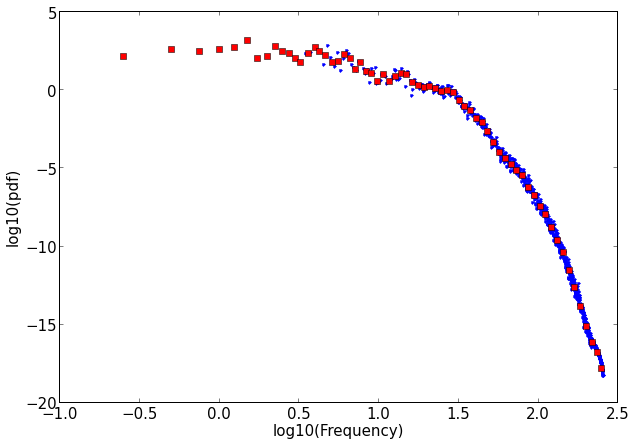
\includegraphics[width=5in]{Figures/binned_EEGpowerspectrum.png}
% \caption{Binned power spectrum}
% \label{binnedEEGpowerspec}
% \end{center}
% \end{figure}

\textcolor{red}{\bf [About here, a short pitch on pink noise is required to set the stage of the great method, and to justify the log log binning]}

Figure \ref{binnedEEGpowerspec} shows, in double logarithmic scale, the original 1024 bins (blue dots) of the pdf obtained from averaging the n power spectra of one sample, and the resulting "compressed"  pdf with 100 log-bins. As we can see, the log-binning preserves very well the structure of the pdf.

In summary, we have built a probability density function of brain frequencies as captured by the Neurosky hardware, from the n power spectra of each sample. We have then used a log-binning method to reduce the 1024 bins from the original power spectrum to an arbitrary smaller number of log-bins (e.g., 100 log-bins on the Figure). This method makes a sort of statistical averaging by stacking, and then ``compresses" the result in way that it is easy to use in a classifier.

{\bf NB:} I believe that the classifier does well because it can efficiently capture the overall level of activity for all log-bins, but also more local deviations. On the figure, we can see some local peaks mostly between $10^1$ and $10^1.5$, but in all other parts of the pdf though in a less visible way. I believe these deviations are quite unique and can make the difference in the classifier. We should indeed check this further if we want to understand to origins of the good results.

{\bf Side note:} one way to investigate further would be to see indeed to what extent the ``compression", i.e. the small number of log-bins, affects the quality of the classifier. Another quite promising further research direction, would be to determine the minimum number of n power spectra, which should be taken into account to reach a target level of correct classification. This would be useful to determine what should be the most adequate sample size for a certain level of identification. This level might of course vary as a function of subjects and tasks.

%-----------

Finally, we create a one-dimensional signal by flattening each bin in the time dimension, computing the mean magnitude of each bin over all readings in the recording. The resulting signal is a one-dimensional row vector with one entry for each each measured frequncy bin.

\textcolor{red}{\bf [Maybe a schema would be great to help the reader get the point quickly]}

From this point, we are equipped with a feature vector of arbitrary size and statistical relevance as an input for our classifier.

\subsection{Classifier}

Support vector machines (SVM) are a set of supervised machine learning methods that take labeled example data to create a model that can be used to predict the classes of unlabeled data. SVMs use a hyperplane (an n-dimensional construct in n+1 dimensional space) to draw discriminatory boundaries between classes. In contrast to linear discriminant analysis, which has a long history of use in BCIs, SVMs select the hyperplane that maximizes distance from the nearest training points, which has been shown to increase the model's generalizability \cite{burges_tutorial_1998}.  For more on SVM's in BCI: \cite{garrett_comparison_2003,grierson_better_2011} 

In this study, we use LinearSVC, \cite{fan_liblinear:_2008} a wrapper for LibLinear exposed in Python through the ScikitLearn library. \cite{pedregosa_scikit-learn:_2011} We chose LinearSVC primarily because its underlying C implementation is very performant, and because linear kernels performed as well or better than nonlinear ones in early experimentation, corroborating the findings of previous studies \cite{garrett_comparison_2003,lotte_review_2007} \textcolor{red}{Please provide evidence if you can}.  We use the default settings for LinearSVC - a C of 1.0, squared hinge loss function, and a tolerance parameter of of 1e-4. \textcolor{red}{You might want to explain what these parameters are, by e.g., providing the main formula of the LinearSVC.}


\subsection{Per-user calibration}

We conducted a simulated calibration step for each participant. For each subject, we generated every possible pair of two tasks and cross-validated our SVM seven times on that subject's recordings for those two tasks. We used ScikitLearn's built-in cross-validation toolkit, which was configured to perform each of the seven cross-validation steps using different splits of trial data in the training and testing sets. For every task pair processed, we recorded mean classification across all cross-validation trials. We repeated this calibration process for all users at every combination of recording length and (log-)bin size. 

As an additional performance audit, we timed our SVM at training time. We fit an SVM to all the data for two task-pairs from two randomly-selected subjects, and repeated this process ten thousand times at different bin sizes and different lengths. We report the minimum time of each ten thousand attempts. In order to establish a proper estimate, we time the SVM after all data has been loaded to memory, disregarding the time it takes to load the data from disk.

\textcolor{red}{[Is this time thing relevant in the sense that some situations really provide a significant gain compared to others?]}

% TODO: we should test at test-time also no?


\section{Results}

\subsection{Classification accuracy}


% TODO: table of best-case at different bin-sizes and times?

Surprisingly, classification was better than chance even at a bin size of y (i.e., when each feature vector in the training and testing sets contained only y features).


{\bf Q. 2.}

    By the way, I generated the average classification performance per subject directly in the spreadsheet. In most cases, we see little decrease in performance vs. bins. Although the accuracy is always above gambling (50\%), some subjects are clearly harder to classify than others. This is maybe an interesting result to discuss further.


% TODO: something about BCI illiteracy!

\begin{figure}
\begin{center}
%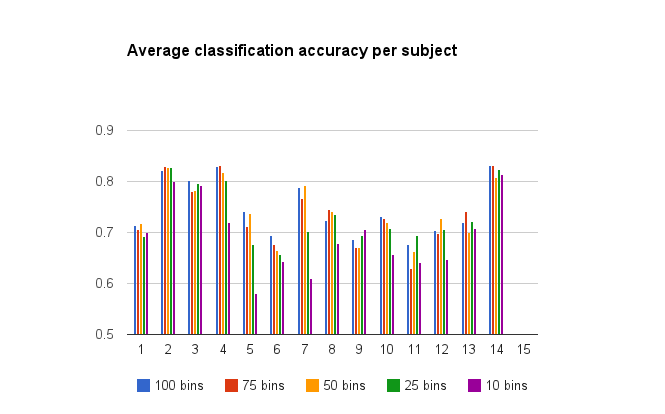
\includegraphics[width=6in]{Figures/avg_classification_accuracy_per_subject.png}
\caption{ }
\label{ }
\end{center}
\end{figure}


i'm wondering if there are a few outlier tasks here - like, a few tasks on which we get very low classification accuracy, dragging down the average
 

{\bf Q. 3.} Related to the average classification accuracy per task pair (second Figure), the difference between task pairs is striking. It seems that all pairs involving ``color" rate high, as well as ``finger" and ``base". However, it's hard to distinguish between ``finger" and ``base" ! I recall that the "color" task is longer than others. I guess it can be a reason for this result \textcolor{red}{\bf [Did you make any correction to take into account only the same sample size, i.e., max 10 seconds?]}. I attached an updated chart with all x-axis labels.

\begin{figure}
\begin{center}
%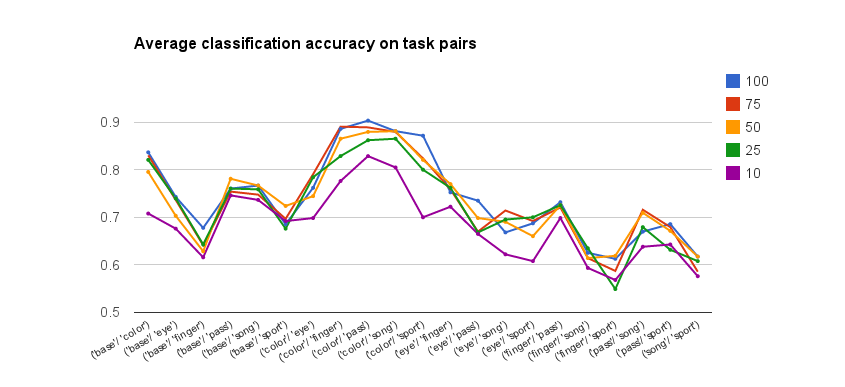
\includegraphics[width=6in]{Figures/avg_classification_accuracy_taskpairs.png}
\caption{ }
\label{ }
\end{center}
\end{figure}


{\bf Q. 5.} I also recall that we have discussed that it would be great to look how long (in seconds) it take to properly classify. Concretely, we have more or less 10 seconds per sample (at the exception of the ``color" task as far as I remember). So instead of classifying on the binned probability density function (pdf) build from an averaging power spectra over 10 seconds, what happens if we classify based on pdfs built on averaging power spectra on 1,2,3,...., and then 10 seconds instead ?




\subsection{Performance}

% TODO: figure of performance versus speed

% TODO: report regression between performance and speed

% TODO: regression on testtime as well?
\section{Discussion}

We find that logarithmic binning dramatically decreases the computational expense of EEG-based calibration and classification without a significant detriment to accuracy. 

Logarithmic binning could enable co-adaptive, online BCI with as few as one dry EEG sensor, making online calibration much more performant on mobile or embedded processors with limited computational resources. Alternatively, since logarithmic dramatically decreases the size of data fed to the classification algorithm, the technique could allow calibration to occur ``in the cloud" - the BCI could pre-process the data on board, bin it, and ship this data to a more powerful server, which could process it online. By some combination of cloud-based and on-board processing, BCIs could gain from the accuracy of computationally expensive analytics without having to perform these computations on-board.

\textcolor{red}{\bf [On on-board versus cloud, you want to outline which part of computations should be on-board, and which part should be in the cloud and why. If you go in this direction, you might also want to justify your design, which requires benchmarking each (sub-)task. My impression is that it's a little beyond this paper as we have not even an acquisition/processing app up and running.]}

\section{Limitations and Future Work}

\bibliographystyle{abbrv}
\bibliography{references}


\end{document}
